%abstract.tex

\begin{appendix}
\chapter{Appendix}

\section{Walkability criteria total overview}\label{Acriteria}
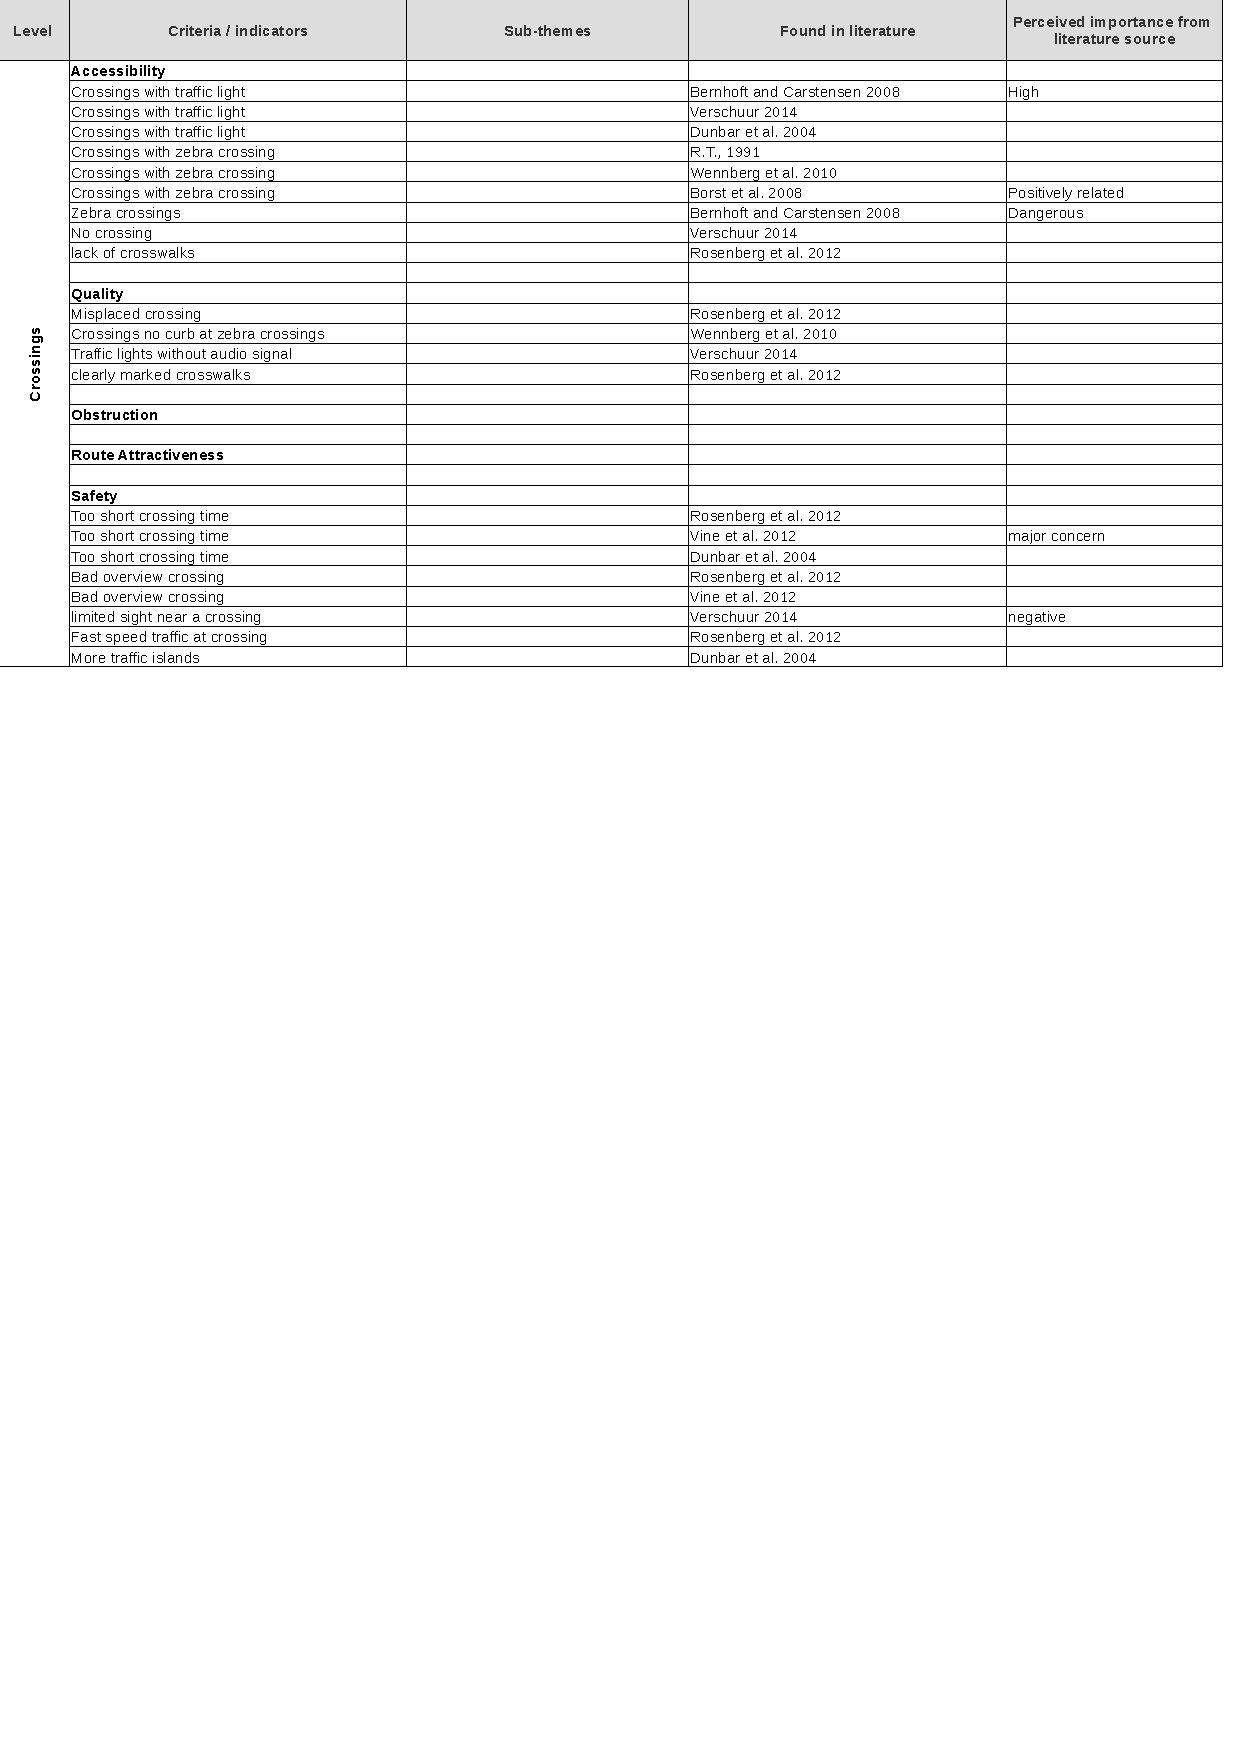
\includepdf[width=\textwidth]{img/annex/A1_crossings_criteria.pdf}
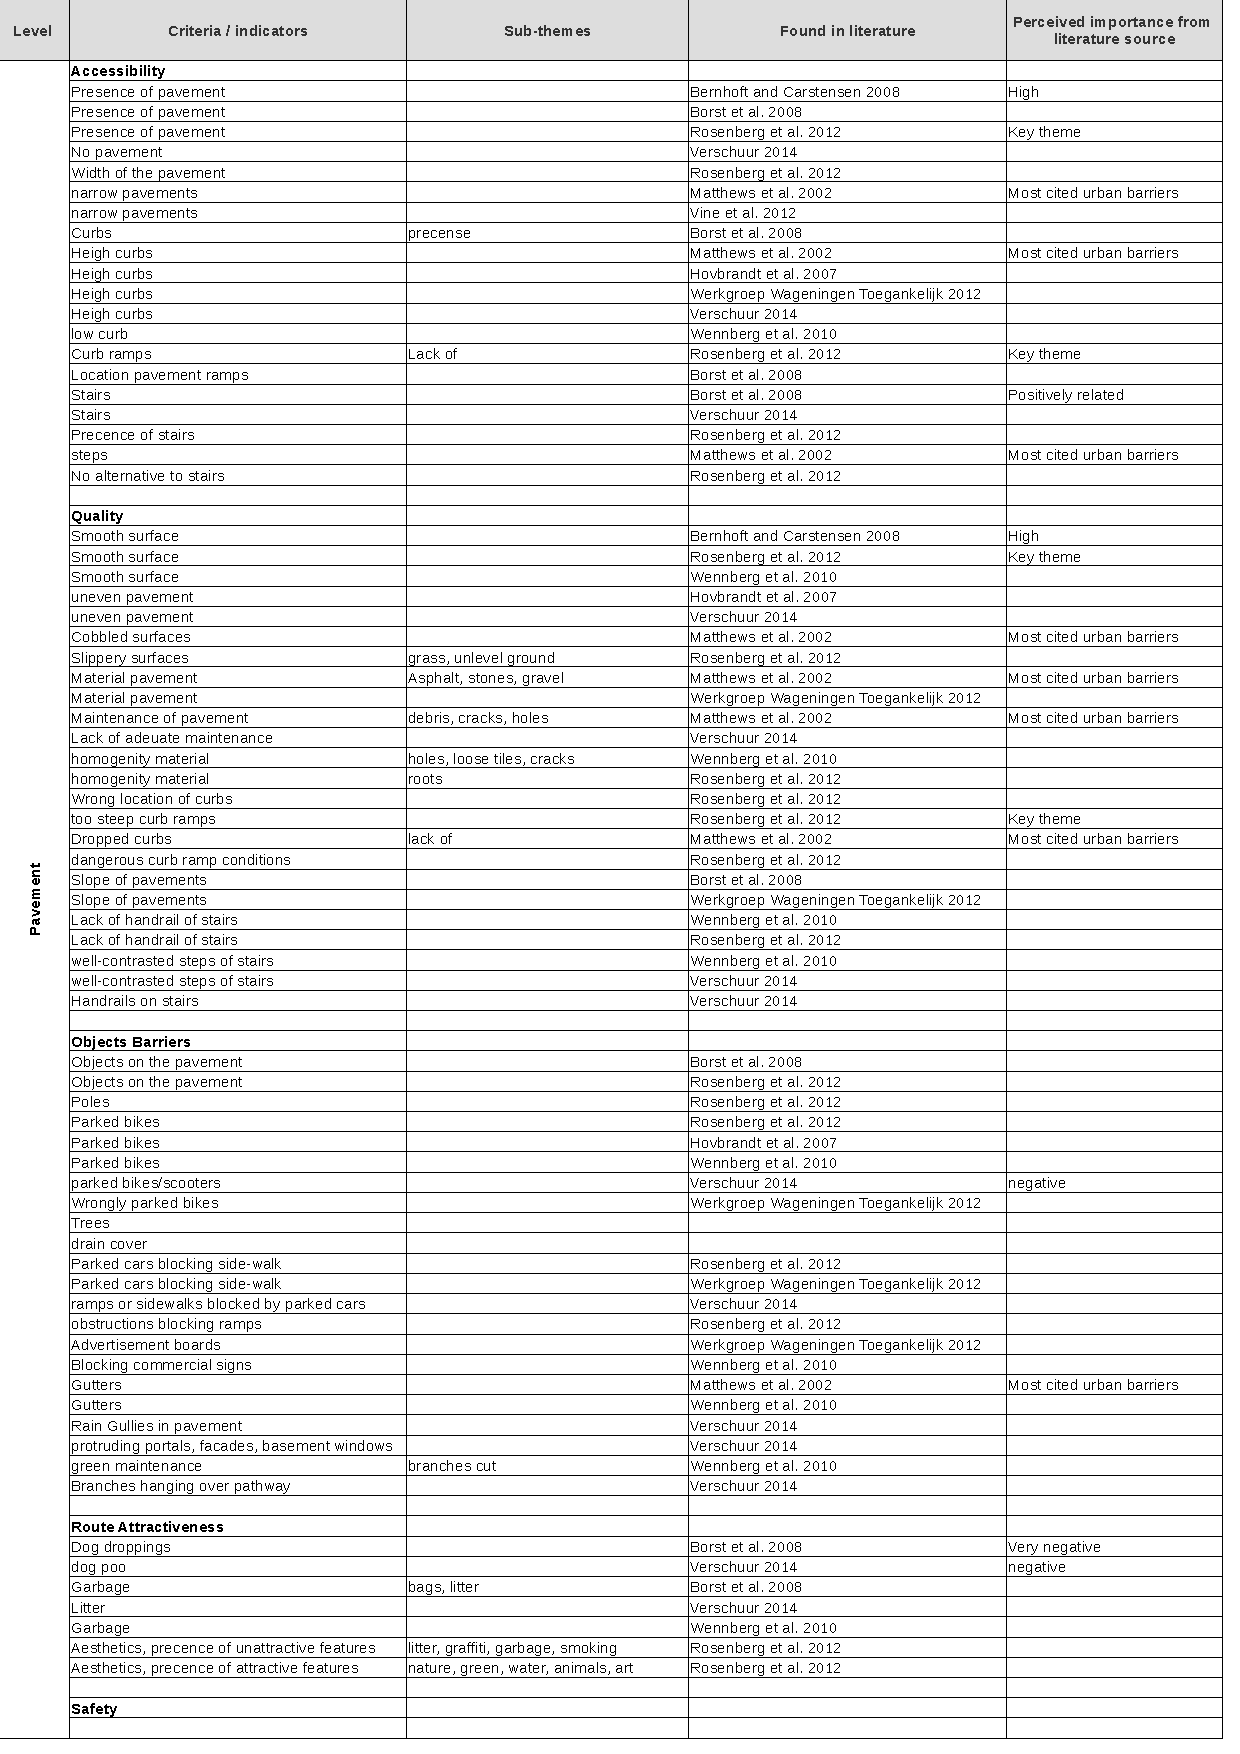
\includepdf[width=\textwidth]{img/annex/A2_pavement_criteria.pdf}
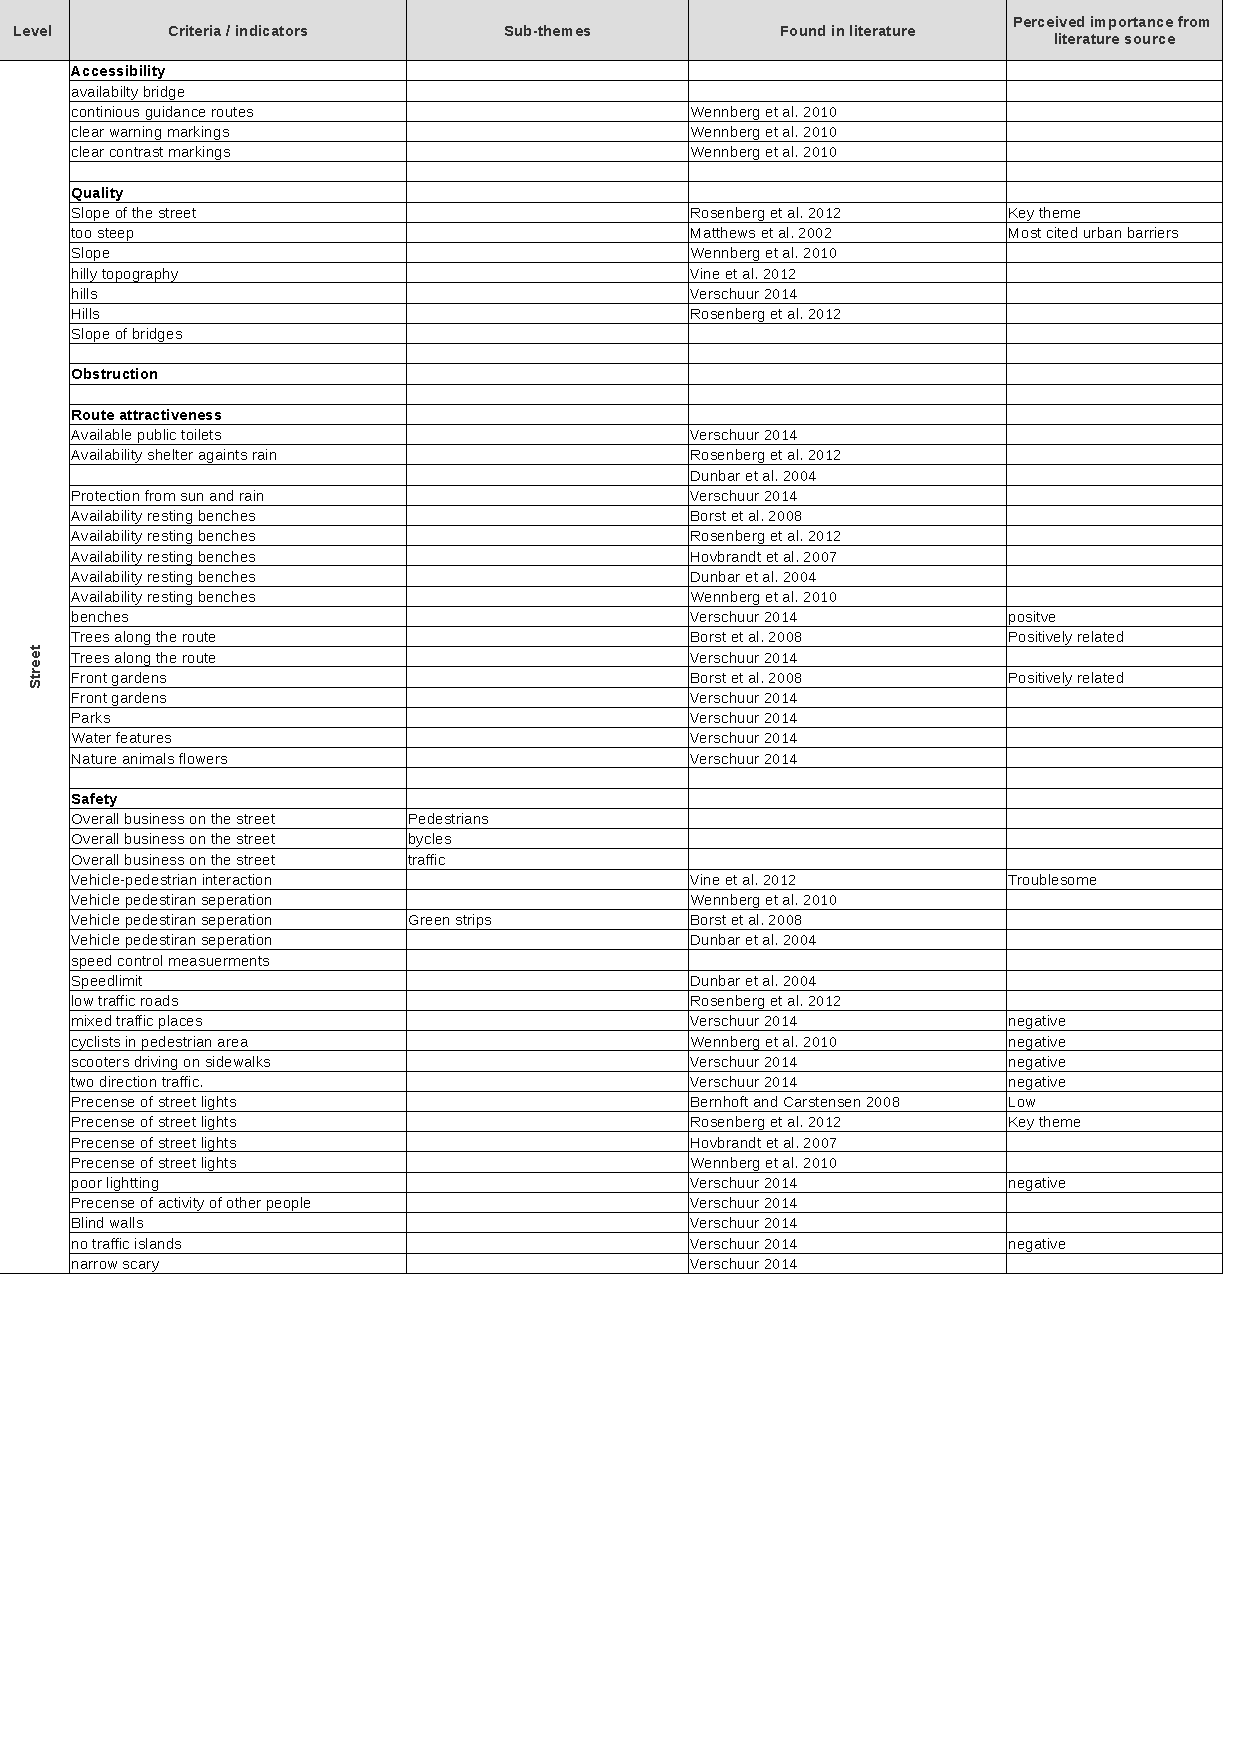
\includepdf[width=\textwidth]{img/annex/A3_street_criteria.pdf}
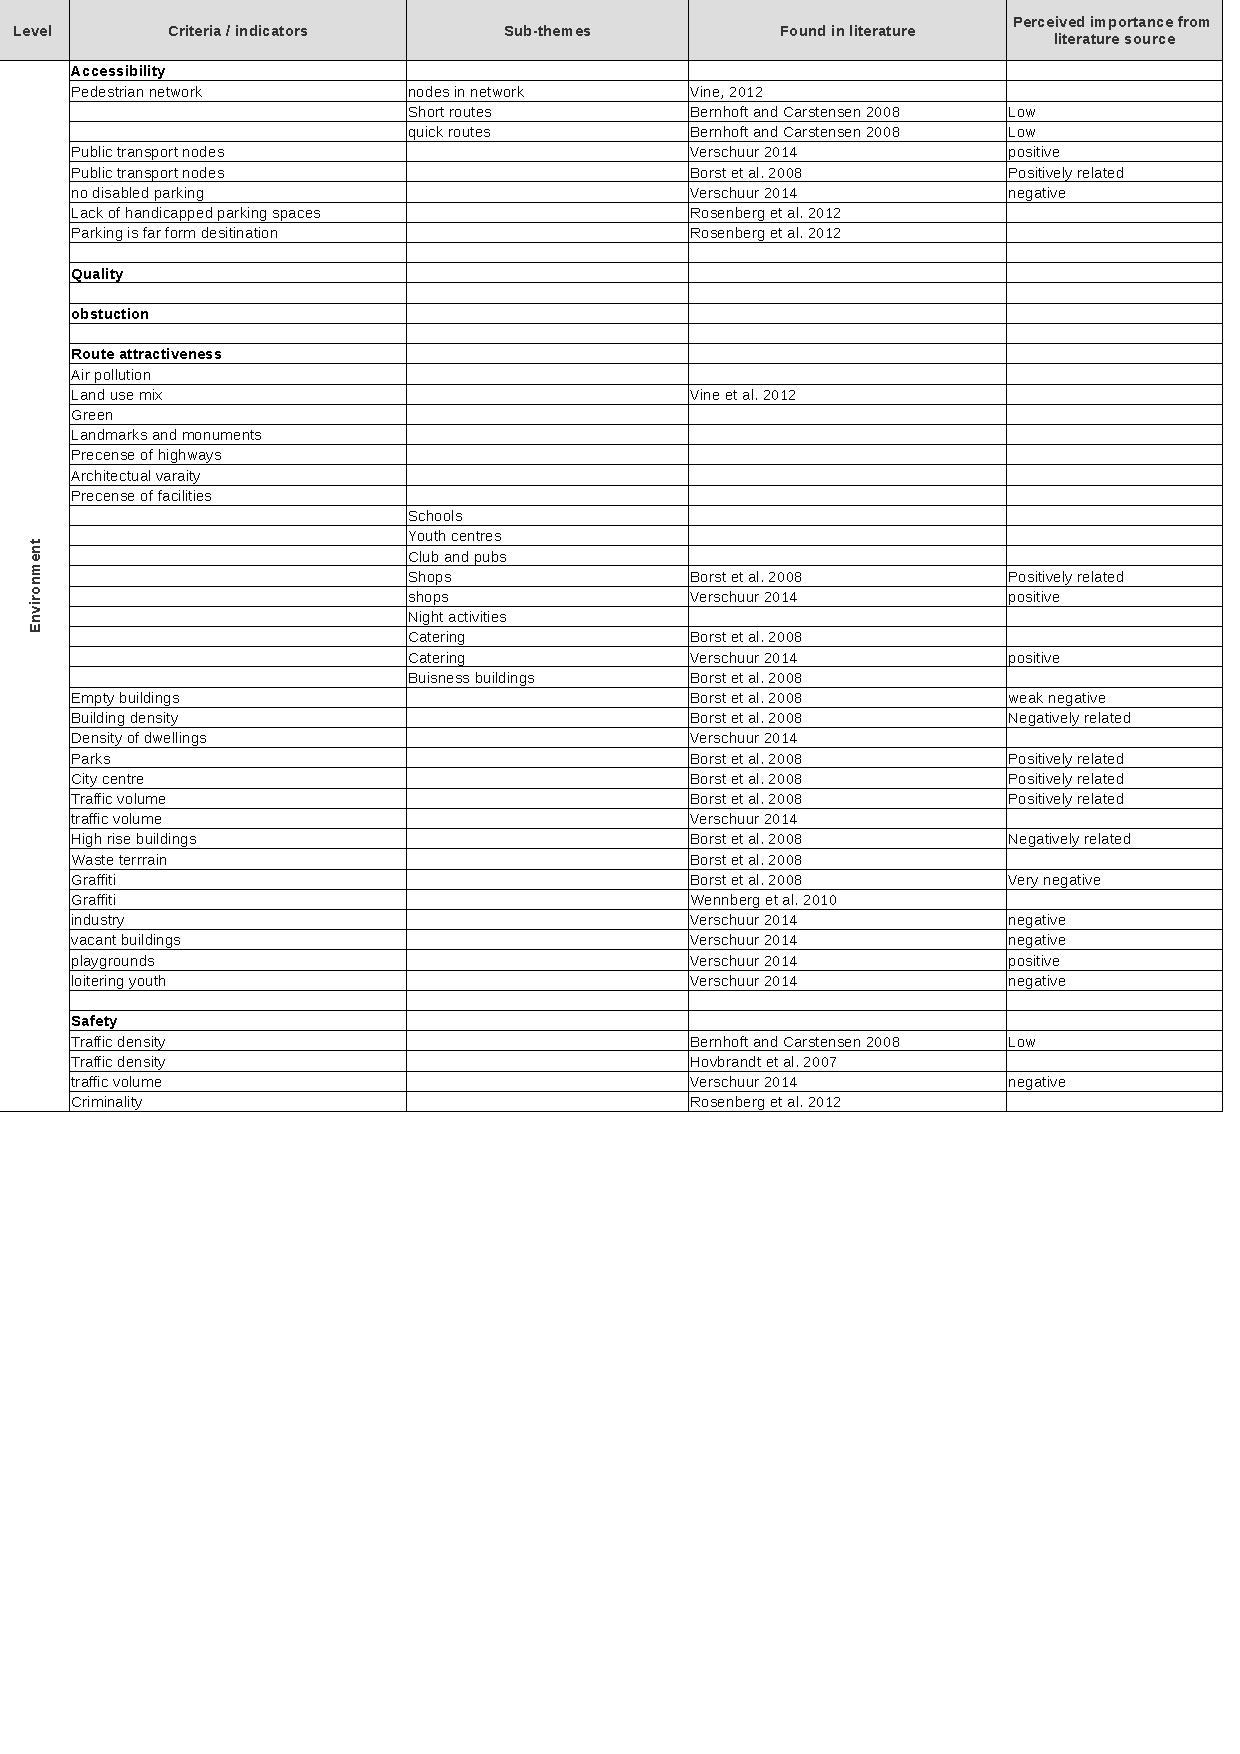
\includepdf[width=\textwidth]{img/annex/A4_environment_criteria.pdf}
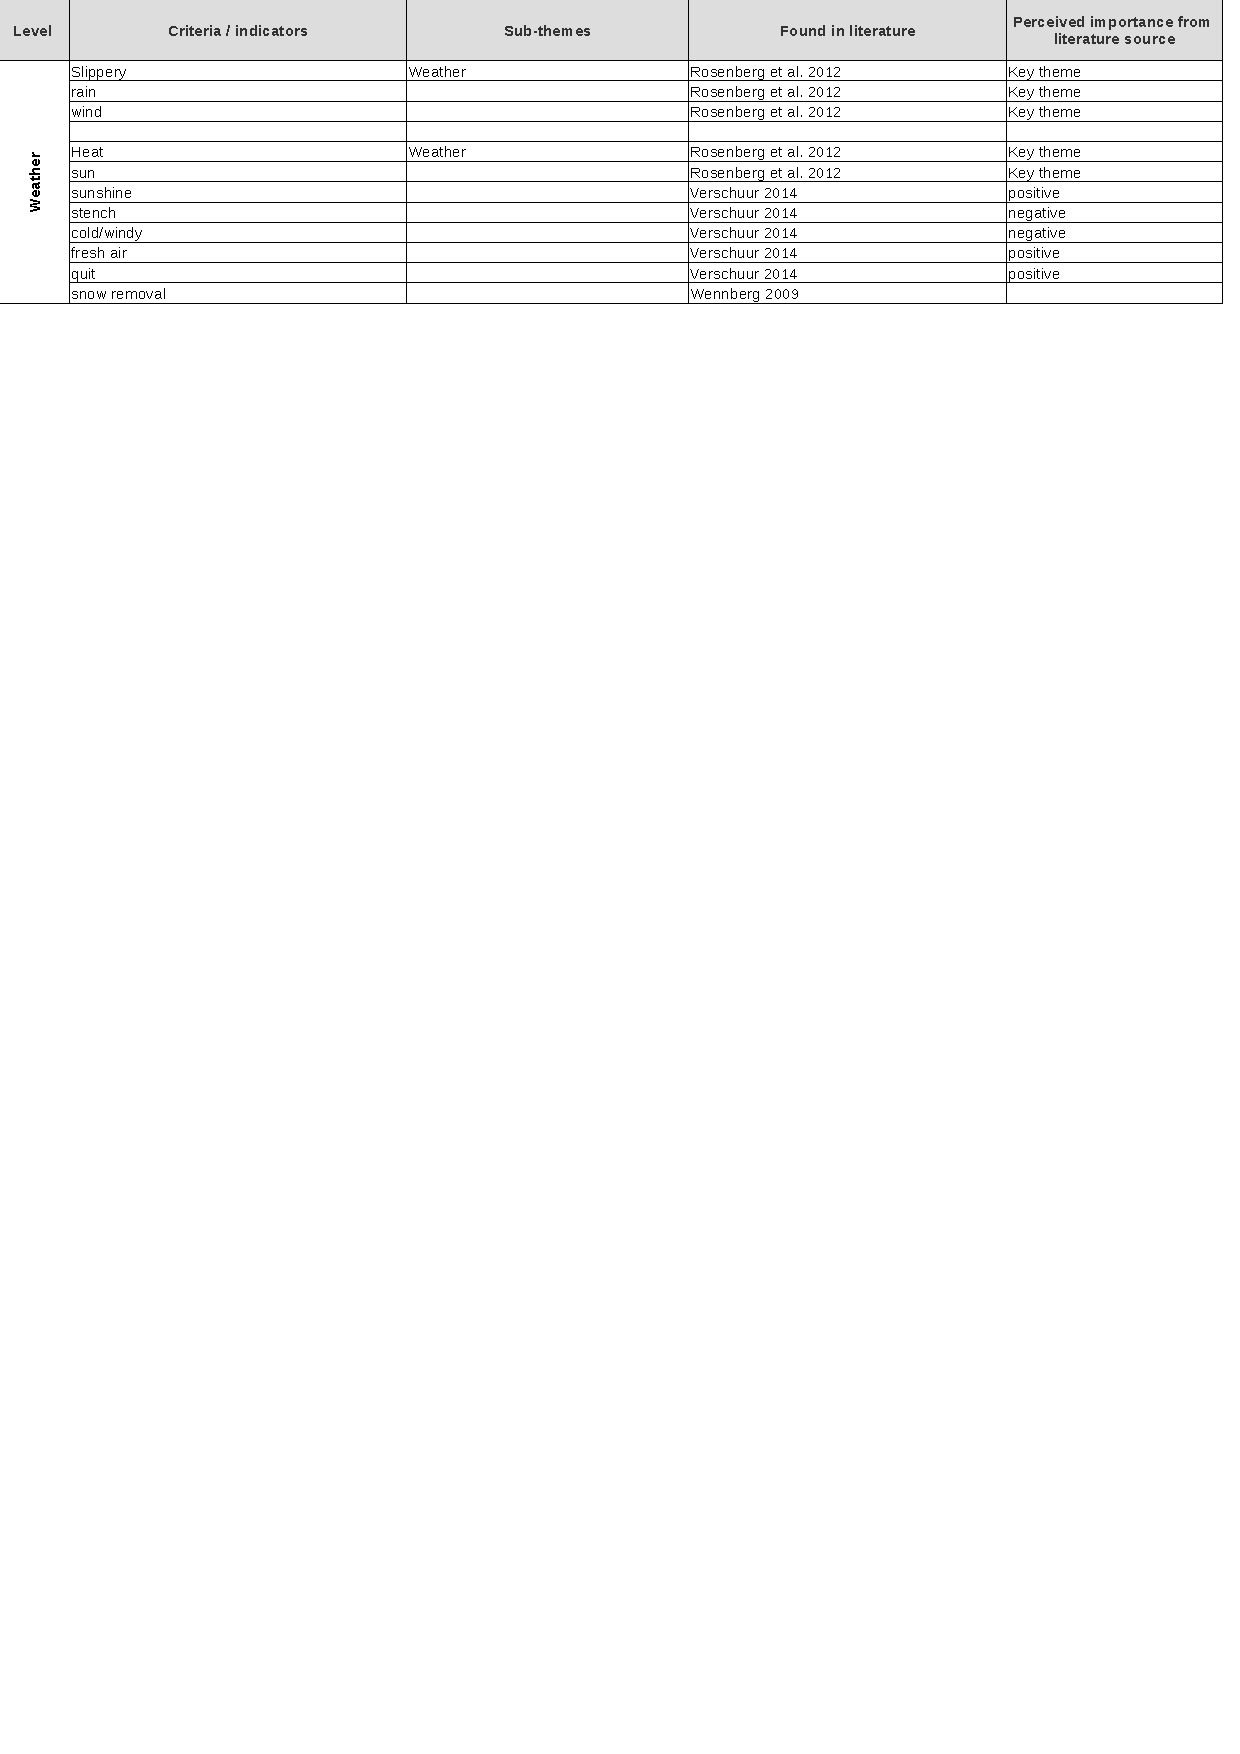
\includepdf[width=\textwidth]{img/annex/A5_weather_criteria.pdf}

\section{Puccini Map Amsterdam}
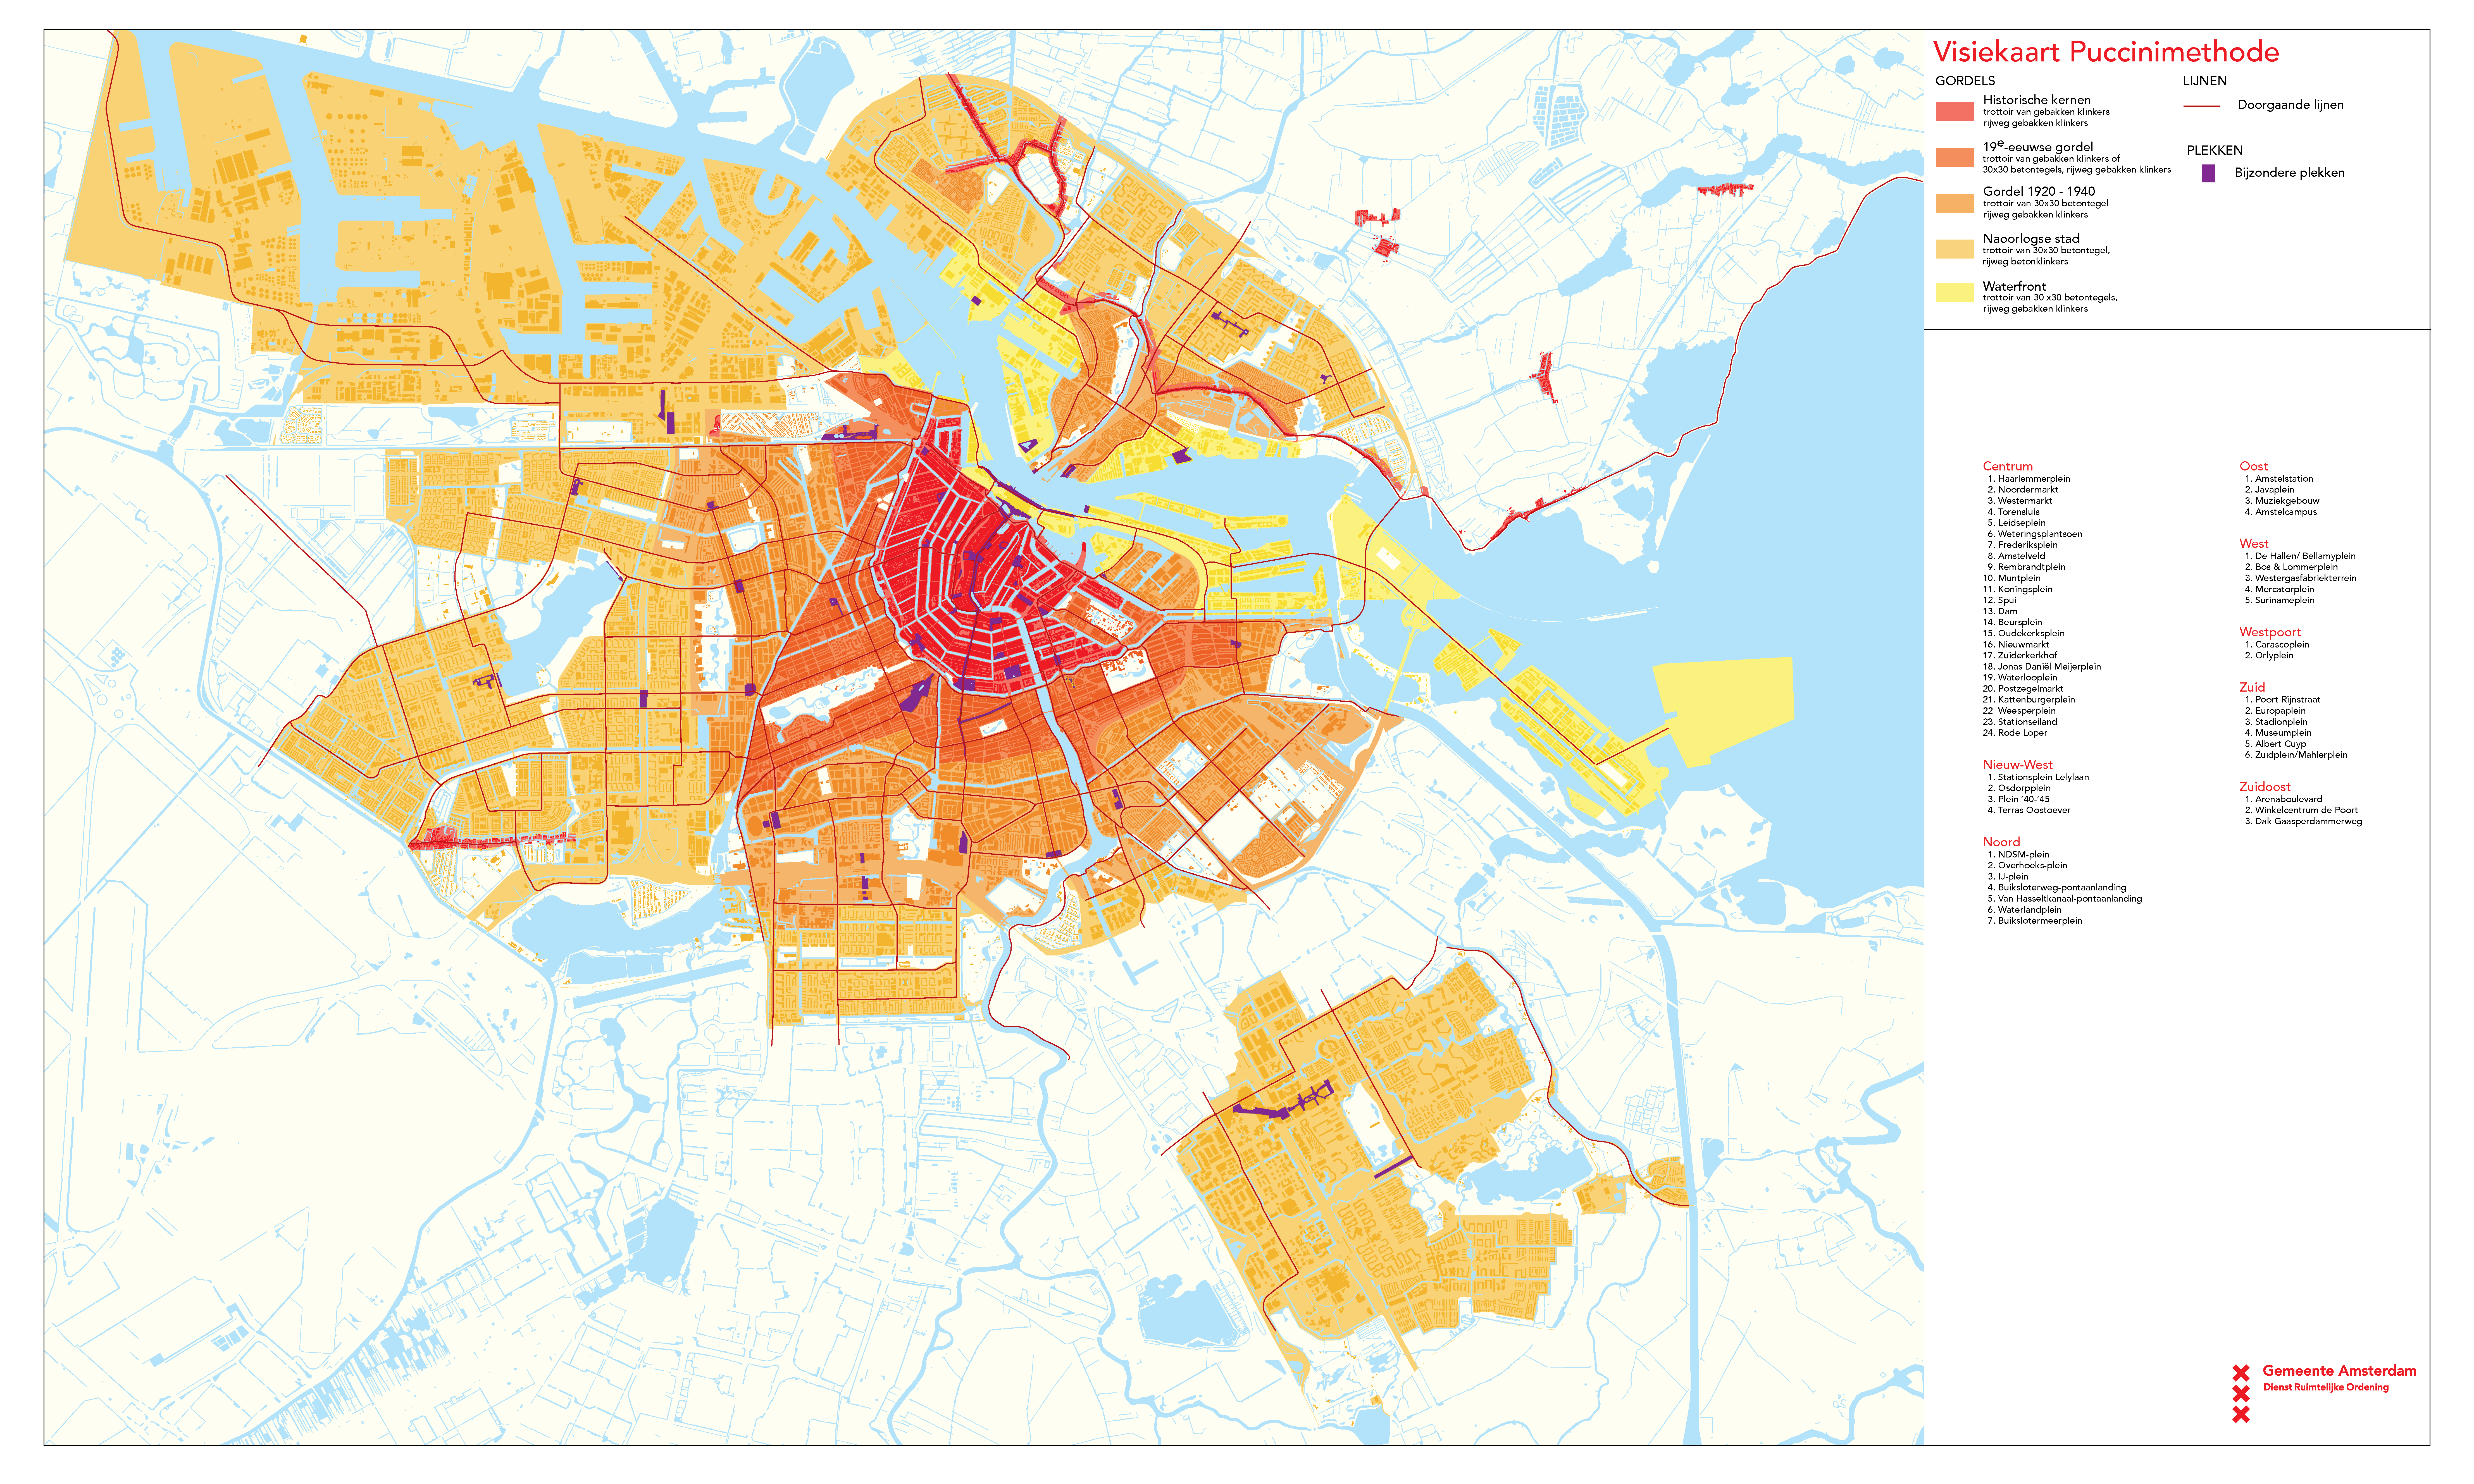
\includepdf[pages=-, scale = 1 , landscape = true ]{img/annex/A_puccini_visiekaart.pdf}\label{pucciniMap}

\clearpage

\section{Questionnaire}\label{Aquest}

\includepdf[pages=-, scale = 1]{img/annex/A_questionaire.pdf}

\clearpage

\section{Accelerometer app alternatives}\label{Aapps}
\textbf{Accelerometer Monitor, Mobile Tools.}
\begin{itemize}
\item Output as .txt file. 
\item Time saved as difference between measurements in milliseconds. No clock-time.
\item $X(m/s^2)$, $Y(m/s^2)$ and $Z(m/s^2)$
\end{itemize}
The Accelerometer Monitor did not give a clock-time bases time stamp, therefore it was hard to link it to the GPS data. Also the .txt output needed some processing before use. 

\textbf{Accelerometer Monitor, keuwlsoft Tools.}
\begin{itemize}
\item Option to safe output on the phone, but only limited amount of readings were done. Then no output was generated any more.
\item Output as .txt file
\item Time as seconds passed. No clock-time
\item $X(m/s^2)$, $Y(m/s^2)$, $Z(m/s^2)$ and $R(m/s^2)$, Theta(deg) and Phi(deg) As given by the application itself. 
\end{itemize}
The Accelerometer Monitor from Keuwlsoft stopped measuring after a random amount of time, so could not be trusted. Also, no clock based time stamp was provided which made it harder to link to the GPS data.

\textbf{AcMeter}
\begin{itemize}
\item No function to save data
\end{itemize}
The AcMeter showed the accelerometer output of the phone on screen, but did not contain a function to save the data. It was not the only application that had only this function, but an example for the many applications that can be found on-line. 

\clearpage

\section{Interviews with elderly list of possible obstacles}\label{Aelderly}
% tabel in annex
% From interviews with elderly list
\begin{enumerate}
	\item = never
	\item = rarely
	\item = sometimes
	\item = often
	\item = always
\end{enumerate}

\begin{table}[ht]
\caption{Average score per possible problem \label{obstacles}}
\begin{tabular}{|l|l|}
	\hline
	 & Average score \\
	\hline
	\multicolumn{2}{|c|}{Quality of the side walk} \\
	\hline
	Bad maintenance of side walks & 4 \\
	Narrow side walks & 1 \\
	too few curb ramps & 3.5 \\
	Sloping side walks & 2.5  \\
	Too steep slopes & 3 \\
	Crossings on bad location & 1 \\
	unclear crossings & 1 \\
	Not enough time for crossing & 2.5 \\
	Mixed use of space & 3 \\
	Bikers on the side walk & 2 \\
	\hline
	\multicolumn{2}{|c|}{Objects} \\
	\hline
	Wrongly parked cars & 4 \\
	Wrongly parked bikes and scooters & 1.5 \\
	Drain covers & 1 \\
	poles on the side walk & 2 \\
	Dog poop & 1 \\
	Not enough resting benches & 1 \\
	Not enough public rest-rooms & 2 \\
	Not enough shelter by rain & 1.5 \\
	protruding portals, facades, basement windows & 3 \\
	\hline
	\multicolumn{2}{|c|}{Overall} \\
	\hline   
	A lot of pedestrians & 3 \\
	A lot of noise & 3 \\
	A lot of traffic & 1.5 \\
	\hline
	\multicolumn{2}{|c|}{Safety} \\
	\hline
	Scary alleys & 1 \\
	Bad lightening by evening/night & 1 \\
	loiterers & 1.5 \\
	Unsafe feeling & 1.5 \\
	\hline
	\multicolumn{2}{|c|}{Environment} \\
	\hline 
	A lack of green & 1 \\
	Bad maintenance & 1 \\
	Ugly buildings & 1.5 \\
	Litter & 1 \\
	Garbage bags & 1.5 \\
	Wind & 1.5 \\
	\hline
\end{tabular}
\end{table}

\clearpage

\section{Failed measurements}\label{Afailed}
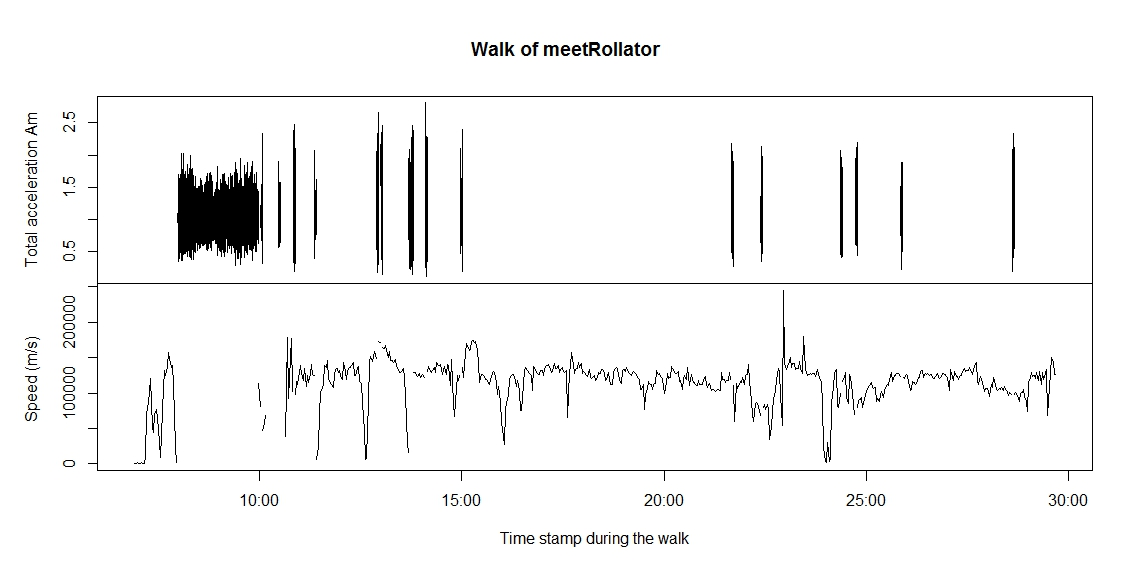
\includegraphics[width=0.85\textwidth]{img/annex/walkmeetrollator.jpeg}
% 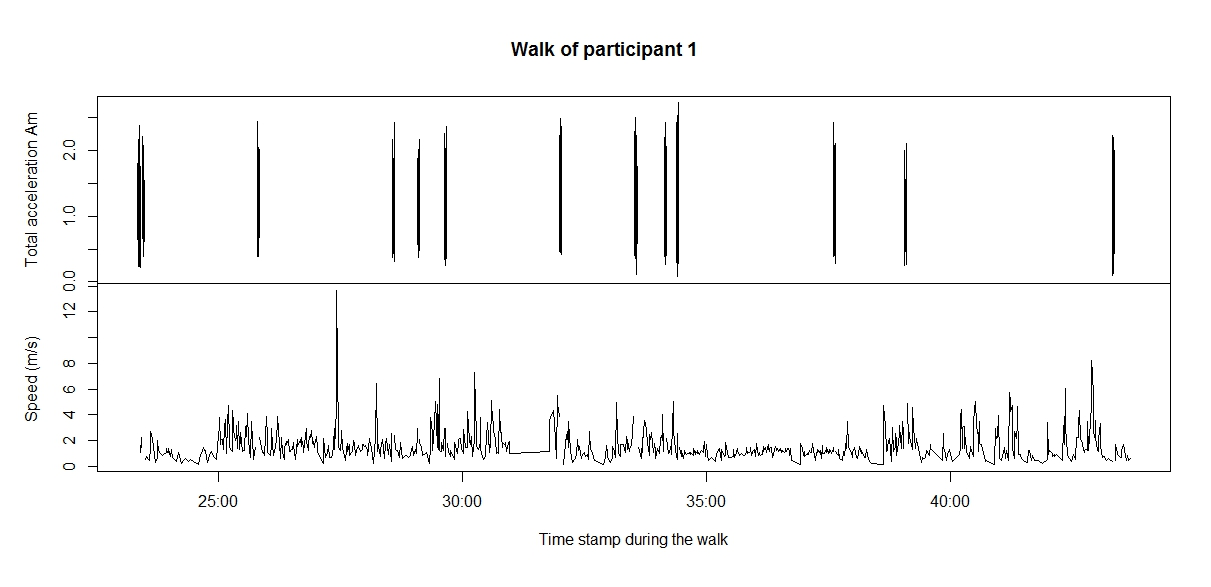
\includegraphics[width=\textwidth]{img/annex/walkpart1}
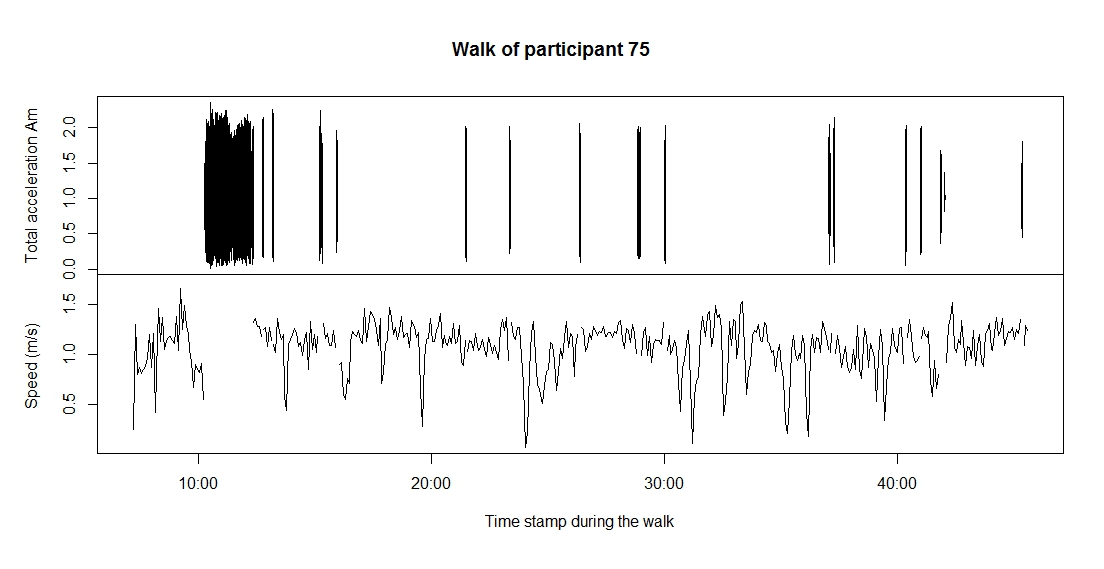
\includegraphics[width=0.85\textwidth]{img/annex/walkpart75.jpeg}
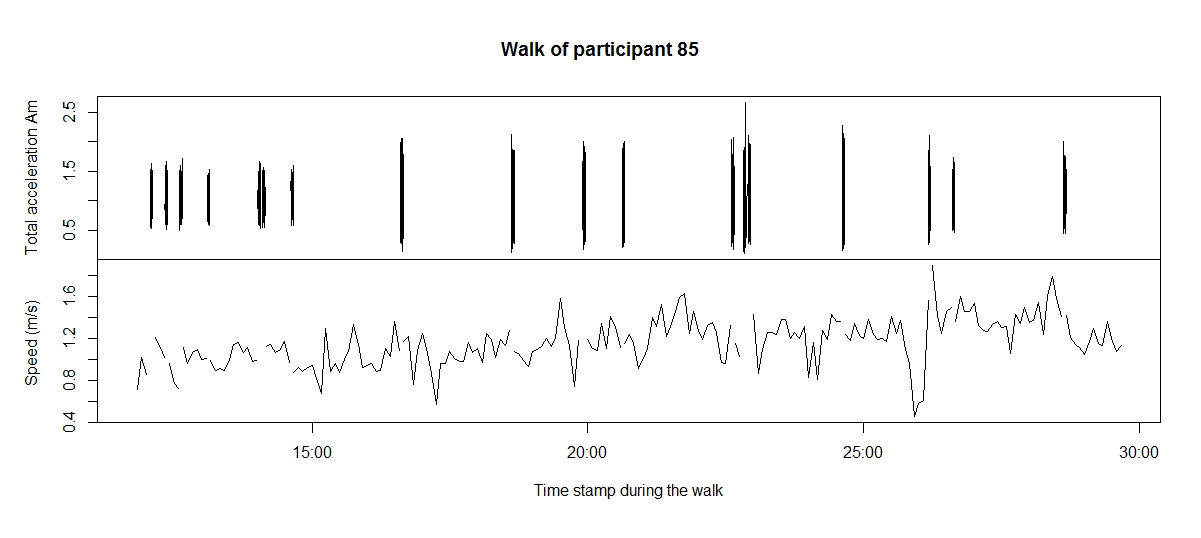
\includegraphics[width=0.85\textwidth]{img/annex/walkpart85.jpeg}
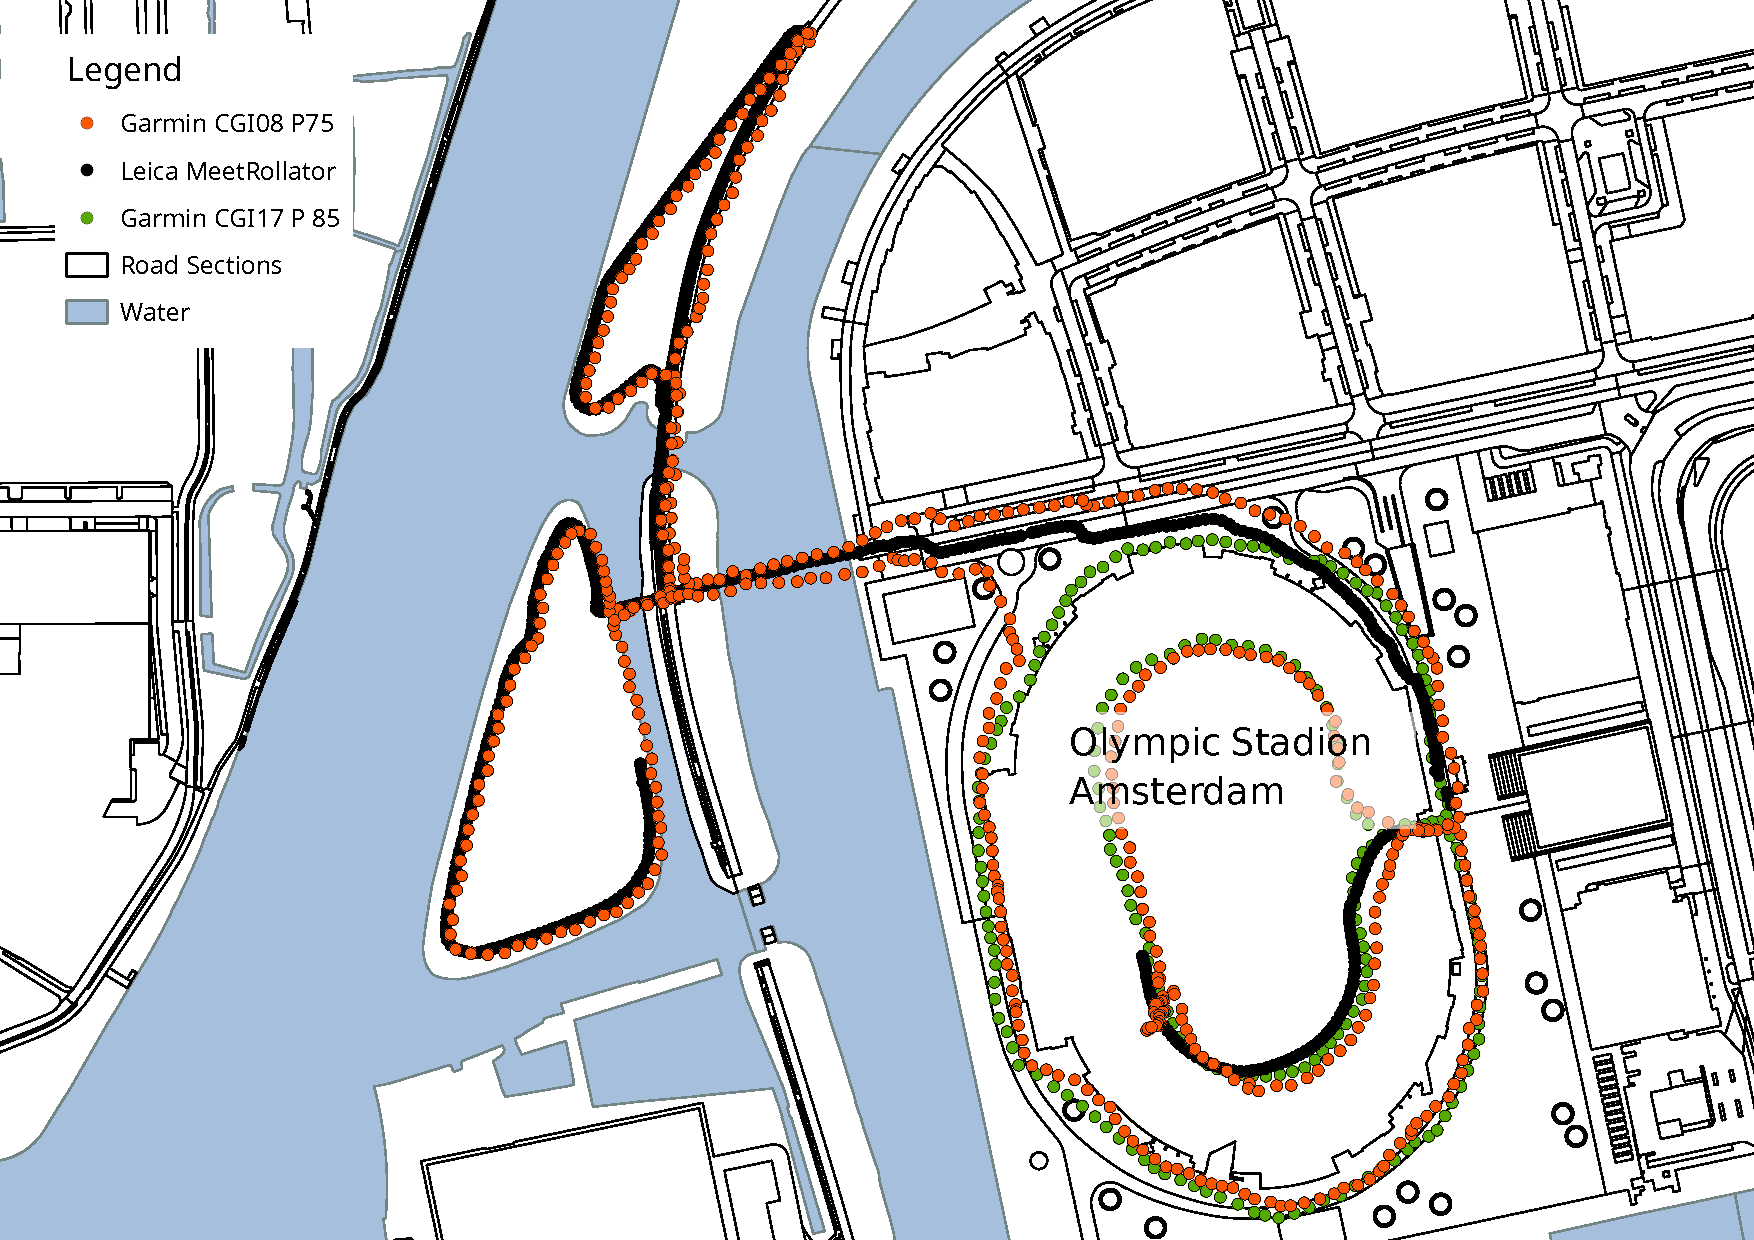
\includegraphics[width=\textwidth]{img/annex/A_failedmeasurementsMap.pdf}

\clearpage

\section{Jordaan road classification total}\ref{Ajordaan}
\includepdf[pages=- , nup=1x1]{img/annex/A_Jordaan_weg_classificatie_resultat.pdf}

\clearpage

\section{Detail of AHN2 of Jordaan}\label{AAHN}
\begin{figure}[h]
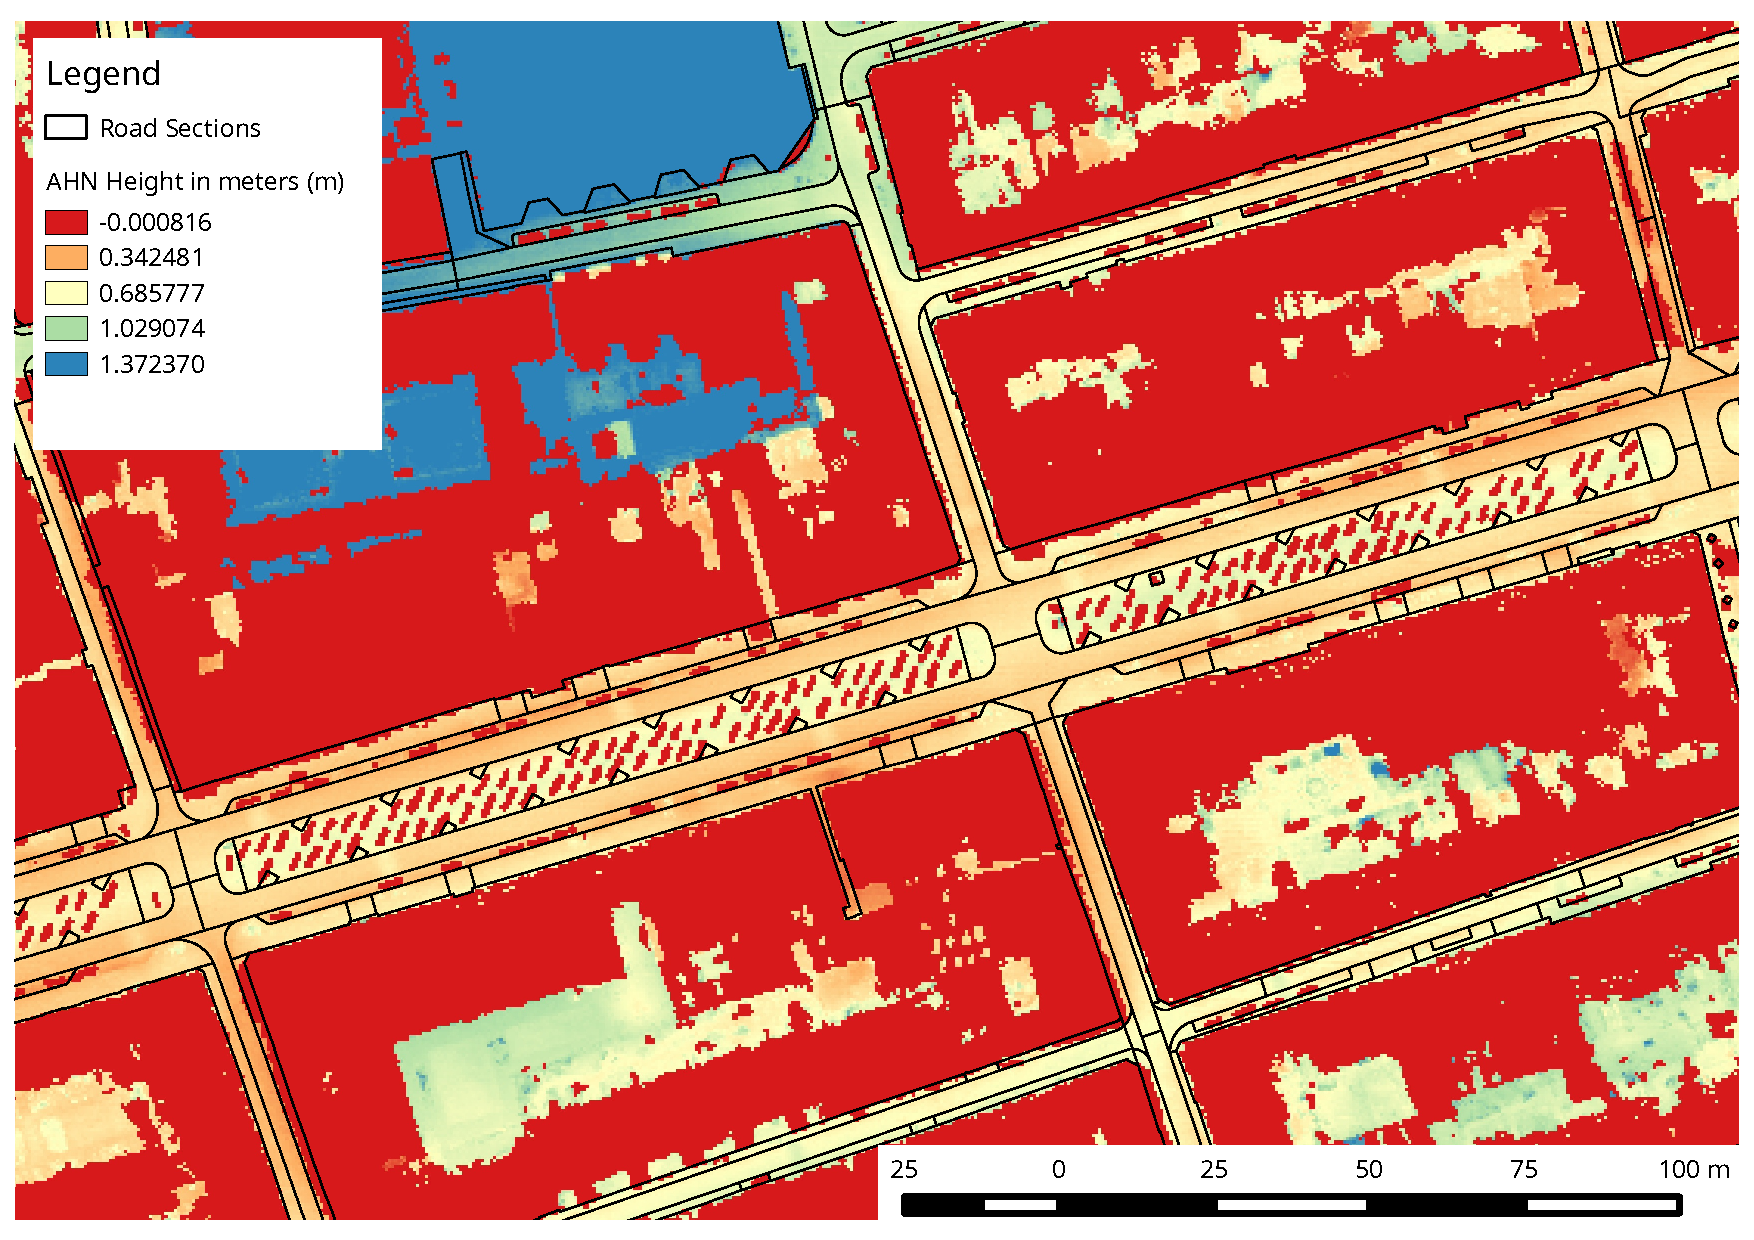
\includegraphics[width=\textwidth]{img/R_AHN_jordaan.pdf}
\centering
\caption{
Detail Jordaan height map\label{jordaanahn}}
\end{figure} 

\clearpage

\section{Change Point methods tests for Speed}\label{Acptest}
\begin{figure}
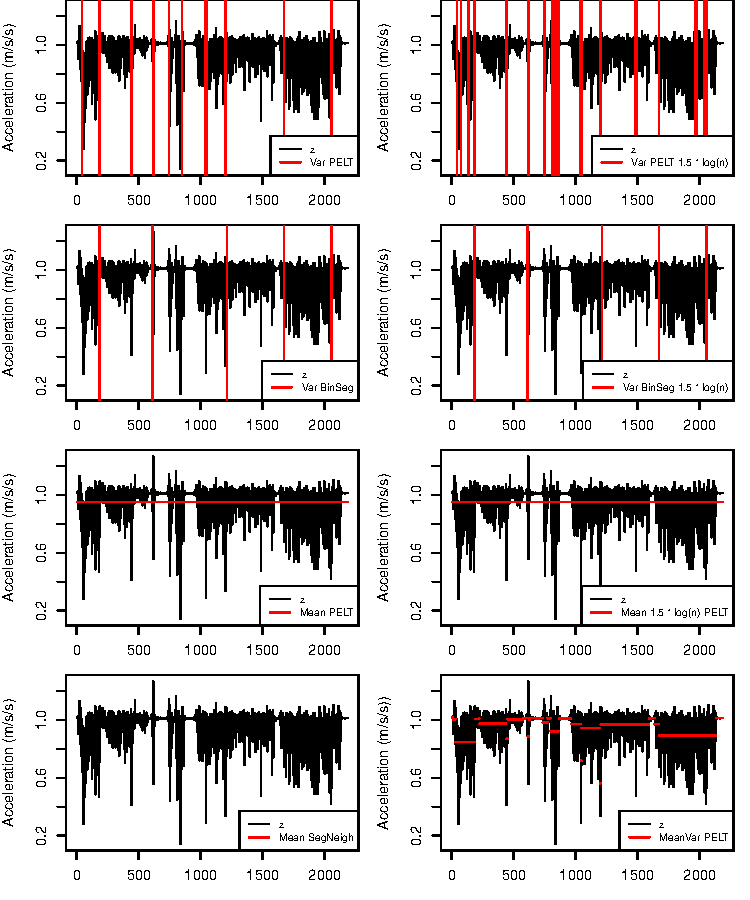
\includegraphics{img/R_comparisonMethodsZax.pdf}
\end{figure}




\end{appendix}